\documentclass[a4paper]{article}
\usepackage[slovene, english]{babel}
\usepackage[utf8]{inputenc}
\usepackage{lmodern}
\usepackage[T1]{fontenc}
\usepackage{fancyhdr}
\pagestyle{fancy}
\lhead{Rok Ivanšek}
\rhead{IŠRM, II}
\usepackage[margin=0.8in]{geometry}
\usepackage{algorithm}
\usepackage{algpseudocode}
\usepackage{amsfonts}
\usepackage{hyperref}
\usepackage{color}

\usepackage{graphicx}
\usepackage{caption}
\usepackage{subcaption}
\usepackage{float}

\title{Cryptography and Computer security\\
Classifying classical ciphers using random forest}
\author{Rok Ivanšek, IŠRM, II}
\date{\today}

% telo dokumenta
\begin{document}



\maketitle


\begin{abstract}
When encrypting a plaintext into a ciphertext, the idea is to hide the actual content of the underlying message, thus making it unreadable for a potential harmful adversary. Ciphertexts are therefore ``gibberish'' texts that do not show any structure that would resemble a natural language. Despite this fact, we can still find patterns in the ciphertexts. The patterns are clearer, when the underlying encryption rule is more transparent, like in the case of classical ciphers. In this report I show that we can use these patterns to match a set of ciphertexts to the corresponding cipher. By carefully engineering features, we can use a random forest technique to train a classifier model that is able to classify ciphertexts of classical ciphers.
\end{abstract}

\section{Introduction and related work}

The hardest part in deciphering a given ciphertext, is to find out what type of encryption was used to produce it. Once this information is known, deciphering becomes a lot easier. By knowing the algorithm that was used, we understand the complexity of the encryption and we can narrow down the methods we will use, to decipher the given ciphertext. Through the recent years statistical classification techniques proved to be extremely successful in a large set of domains, such as computer vision, speech recognition, handwriting recognition, natural language processing and many more. In this assignment we use statistical classification, in particular the ensemble method called random forest \cite{breiman2001random}, to try and build a model that is able to distinguish between different classical ciphertexts. An accurate classification model would help a lot in the early stages of deciphering ciphertexts and may save countless hours of time for a cryptologist. In the domain of ciphertexts, classification has been attempted for classical substitution ciphers using a neural network by Sivagurunathan, Rajendran and Purusothaman \cite{sivagurunathan2010classification}, modern block ciphers like DES, 3DES and AES using support vector machines by Dileep and Chandra Sekhar\cite{dileep2006identification}. Another approach was used by Maheshwari \cite{maheshwari2001classification} for both classical and modern ciphers. In \cite{mishra2013pattern} Mishra and Bhattacharjya used a combination of different methods to classify modern block and stream ciphers and a clustering study was done for ciphers from the finalists of the AES contest in 2000 by Souza, Tomlinson, Figueiredo and Luiz \cite{decipher}. In our study we follow a typical data science pipeline and we describe it in detail in each section of this report. First we generate training data by encrypting common plaintexts with different classical encryption techniques. We describe this process in section \ref{data}. Then we engineer features. We describe which features were used and the reason behind it in section \ref{features}. We do some simple exploratory data analysis and present the results in section \ref{explore}. Next we train and tune the model and give a short description of the random forest technique in section \ref{model}. And in the end we present and interpret the results of the classification in section \ref {results}. In addition to the mentioned sections we describe the framework and comment on the work in section \ref{frame_conclusion}.

\section{Data} \label{data}

%TODO: Write a short intruduction to data section.

\subsection{Plaintexts}
For plaintexts we randomly choose 1000 texts from the 20 Newsgroups dataset. We used the preprocessed dataset from \href{http://ana.cachopo.org/datasets-for-single-label-text-categorization}{Ana Cardoso Cachopo} \cite{2007:phd-Ana-Cardoso-Cachopo}. The preprocessing made on original texts from the 20 Newsgroups dataset was:

\begin{itemize}	
	\setlength\itemsep{-0.2em}
    \item substitute TAB, NEWLINE and RETURN characters by SPACE,
    \item keep only letters (that is, turn punctuation, numbers, etc. into SPACES),
    \item turn all letters to lowercase,
    \item substitute multiple SPACES by a single SPACE,
    \item the title/subject of each document is simply added in the beginning of the document's text.
\end{itemize}


In addition to the preprocessing already made, we take out the white spaces and trim the texts to length of $500$ characters. This way we get $1000$ strings of length $500$, each representing a part of a randomly selected text from the dataset. This strings were the plaintexts used in the analysis.

\subsection{Ciphertexts}
To encrypt the plaintexts we use the python library pycipher \cite{pycipher}. To make the classification task as representative as possible, a variety of different ciphers is chosen. Some would produce similar ciphertexts, like the Permutation and Caesar cipher and some ciphertexts, that are clearly distinguishable from each other, like the ADFGVX and the Vigenere cipher. While encrypting, the key of the cipher was always chosen randomly out of all possible combinations, except where stated differently. Each plaintext was encrypted with every chosen cipher. This way we obtain $6000$ cipherthexts, a $1000$ for each of the chosen ciphers. The following ciphers were chosen.\\
\\
In the description of the ciphers we always assume that $x = (x_{1}, x_{2}, ...,x_{m})$ is a plaintext consisting of $m$ integers from ring $\mathbb{Z}_{26}$ which map to letters in the english alphabet.

\subsubsection{Affine cipher}
The affine cipher is in essence a standard substitution cipher, meaning that each letter encrypts to one other letter. The key are integers $a$ and $b$. The encryption rule is
$$e(x_{i}) = (ax_{i} + b) \;\bmod\; 26, \forall i$$
where $a$ is relatively prime to $26$ and $b$ is an arbitrary integer in $\mathbb{Z}_{26}$.

%http://www.practicalcryptography.com/ciphers/affine-cipher/
%https://en.wikipedia.org/wiki/Affine_cipher

\subsubsection{Vigenere cipher}
The Vigenere cipher originates from the 16th century. It encrypts the ciphertexts in blocks of $n$ characters. For a chosen keyword $K = (k_{1}, k_{2}, ..., k_{n})$ of length $n < m$, it encrypts the plaintext following the rule
$$e(x_{1}, x_{2}, ...,x_{m}) = (x_{1}+k_{1}, x_{2}+k_{2}, ..., x_{n}+k_{n}, x_{n+1}+k_{1}, ...,x_{2n}+k_{n}, x_{2n+1} + k_{1}, ...),$$
where all $+$ operations are done in $\mathbb{Z}_{26}$.

\subsubsection{ADFGVX cipher}
The ADFGVX was a field cipher used by the German Army during World War I. It uses a modified Polybius square and a single columnar transposition to encrypt the plaintext. The cipher can encrypt all letters of the alphabet and numbers from $0$ to $9$. It uses two keys. First one is used to build a Polybius square and the second one is used for the columnar transposition. The complete procedure of encryption is as follows:
\begin{itemize}
	\item Using the first key, a $6X6$ square is filled with letters and numbers, each column and row represents one of the ciphertext letters A,D,F,G,V or X. This way each letter in the alphabet and the numbers $0$ to $9$ are mapped in a one to one correspondence to pairs of ciphertext letters. This way we get a ciphertext twice as long as the plaintext and only consisting of ciphertext letters.
	\item To further encrypt the ciphertext obtained in the first part, we use the second key. We write down the ciphertext in rows under the second key and than sort the columns of the obtained table, so that the letters in the second key are in alphabetic order. Following this, we write down the letters from the sorted table column by column, to obtain the final ciphertext.
\end{itemize} 
The important properties of the ADFGVX cipher are that it uses only the letters A,D,F,G,V and X in the ciphertexts and that the ciphertext is two times as long as the plaintext. You can read more about this cipher in \cite{practicalCrypto}.

\subsubsection{Caesar cipher}
The Caesar cipher is one of the earliest known and simplest ciphers. It is a shift cipher that shifts all the letters in the plaintexts by a key value $k$. It can be viewed a special case of the Vigenere cipher, where the key is of length $1$. The encryption rule is
$$e(x_{i}) = (x + k) \;(\bmod\; 26), \forall i.$$

\subsubsection{Permutation cipher}
Also called the simple substitution cipher, it has been in use for many hundreds of years. It basically consists of substituting every plaintext character for a different ciphertext character. It differs from the Caesar cipher in that the cipher alphabet is not simply the alphabet shifted, it is completely jumbled. The key for this cipher is simply a jumbled alphabet. For example a key $k = AJPCZWRLFBDKOTYUQGENHXMIVS$ would impose the following encryption rule
$$ABCDEFGHIJKLMNOPQRSTUVWXYZ \rightarrow AJPCZWRLFBDKOTYUQGENHXMIVS,$$
meaning a letter in the left string would encrypt into a letter in the right string that is in the same place. For example $M$ would encrypt to $T$.

\subsubsection{Playfair cipher}
The Playfair cipher is a digraph substitution cipher from the 19th century that was also used in the World War I by the British forces. It encrypts pairs (digraphs) of letters using a key square. The full description of the encryption is too long to include in this report. Read more about this cipher in \cite{practicalCrypto}.

%\textcolor{red}{TODO: Add descriptions if necesary.}


\section{Feature engineering} \label{features}
%The first idea was to just use letters in a ciphertext as features (the first letter is the first feature, the second letter the second feature, etc...) and than use deep learning (a neural network with a lot of hiddent layers) as the model. Hopefully the neural network would discover some interesting patterns and correlations in the data, that would allow it to distinguish beetween different ciphertexts. Setting up such a network is not an easy task and there is no guarantee that this method will work either, since it has not been tried in this domain yet to my knowledge. So after some initial runs of the neural network and getting really bad results I focused on engeniring useful features that would make the job easier for the classfier. \\
In order to express patterns in the ciphertexts we have to come up with interesting features. A feature is in essence any property of the ciphertexts that can be expressed in a qualitative or a quantitative way. The features that we decided to use are closely related to the properties of the chosen ciphers. They are mostly quantitative measurements that are used, when one attempts to break the chosen ciphers.

\subsection{Distribution of letters}
The first most simple group of features one can extract is the distribution of letters. This just means that we count, how many times each letter appears in the ciphertext. This way we obtain $26$ features, one for each letter in the alphabet. Using only this simple group of features we would already be able to distinguish between some of the ciphers that use only a subset of letters from the alphabet, like the ADFGVX from other ciphers that use the whole alphabet.

\begin{figure}[H]
    \centering
    \begin{subfigure}[h]{0.5\textwidth}
    		\centering
        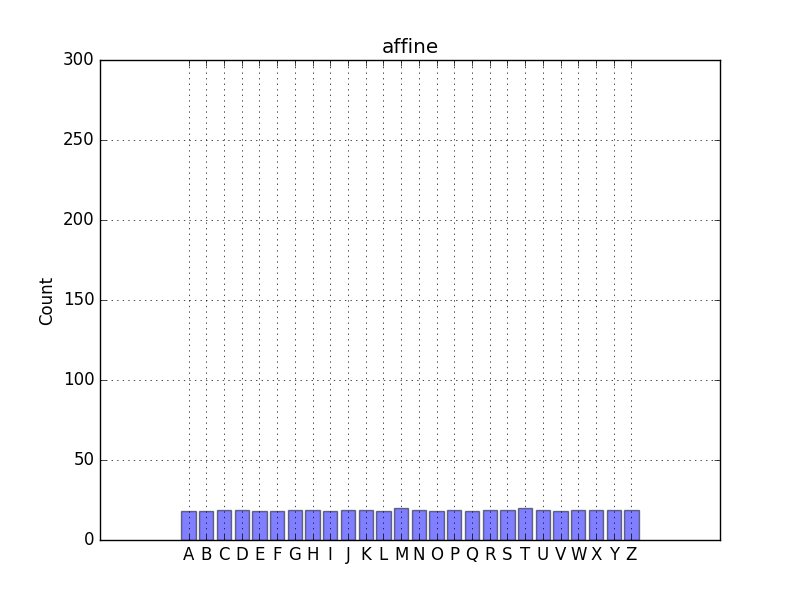
\includegraphics[height=2.5in]{img/affine_dist.png}
    \end{subfigure}%
    ~
    \begin{subfigure}[h]{0.5\textwidth}
	    \centering
        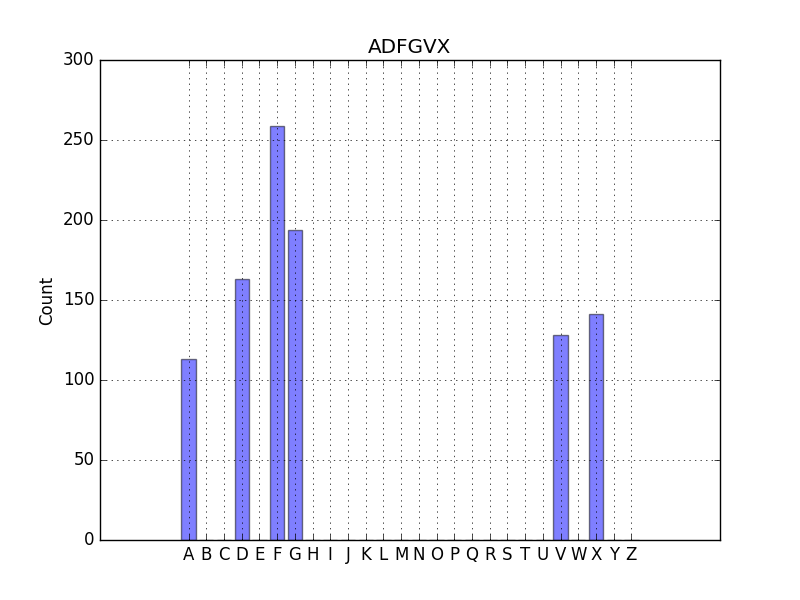
\includegraphics[height=2.5in]{img/adfgvx_dist.png}
    \end{subfigure}
    \caption{Average distribution of letters in the ciphertexts for the Affine cipher (left) and the ADFGVX cipher (right).}
    %\cite{g2:NPMP_prosojnice_mraz_biomodeliranje}}
    \label{fig:letter_dist}
\end{figure}

\subsection{Adjacent duplicates}
Another simple feature that proved to be efficient in a similar ciphertexts classification task \cite{sivagurunathan2010classification} is the number of adjacent duplicates. It is particular useful when recognizing the Playfair cipher, since this cipher should have a substantially lower number of adjacent duplicates than other ciphers, due to its encryption rule.

\begin{figure}[H]
    \centering
    \begin{subfigure}[h]{0.5\textwidth}
        \centering
        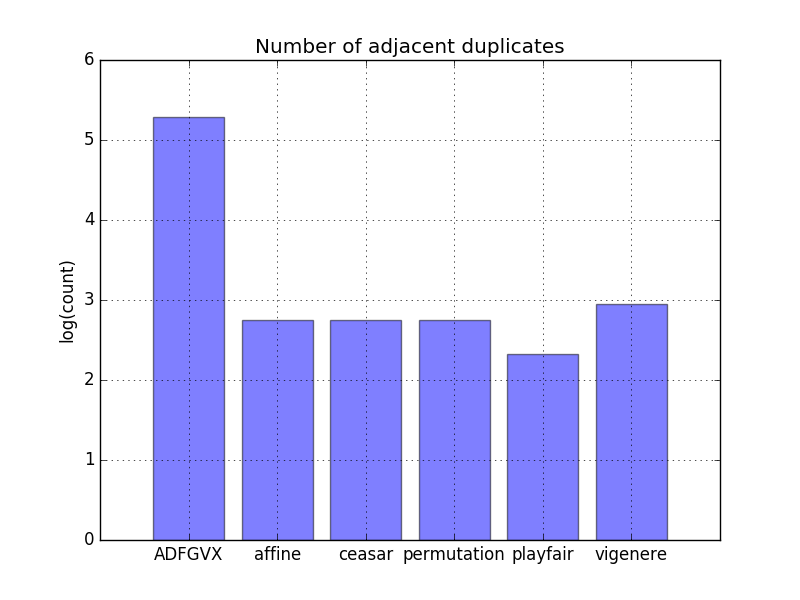
\includegraphics[height=2.5in]{img/no_adj_dups_log.png}
    \end{subfigure}
    \caption{Logarithm of the average number of adjacent duplicates for the used ciphers.}
    \label{fig:adj_dups}
\end{figure}

\subsection{Repeating bigrams}
In a classical text classification an $n$-gram (usually a bigram) is a sequence of $n$ adjacent tokens in a text. Tokens can be words, syllables or letters. Using bigrams of letters I extracted two features. First was the number of unique bigrams that repeat at least once in a ciphertext and second was the frequency of the most frequent bigram in a ciphertext.

\begin{figure}[H]
    \centering
    \begin{subfigure}[h]{0.5\textwidth}
    		\centering
        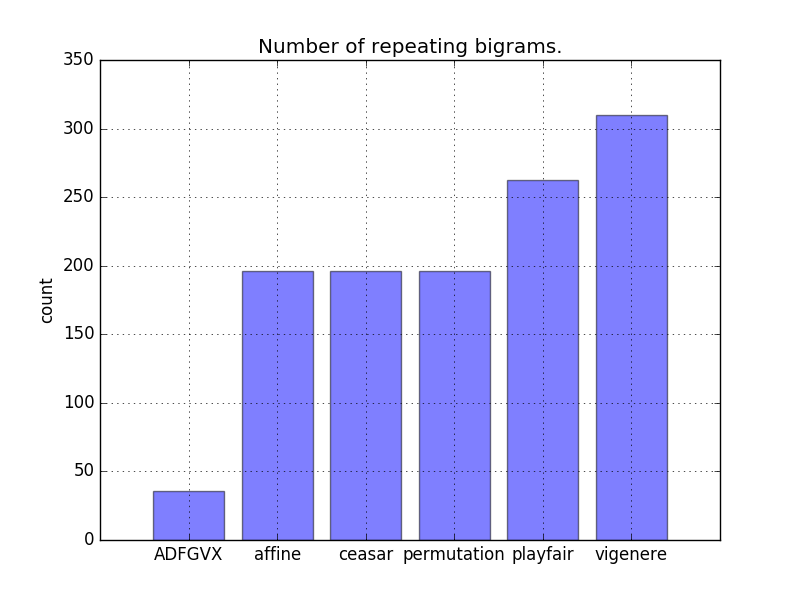
\includegraphics[height=2.5in]{img/bigrams_1.png}
    \end{subfigure}%
    ~
    \begin{subfigure}[h]{0.5\textwidth}
	    \centering
        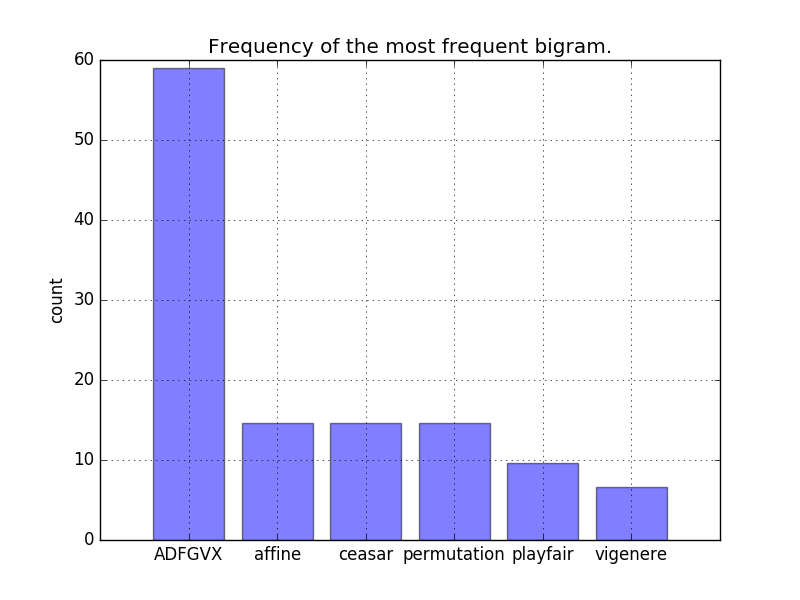
\includegraphics[height=2.5in]{img/bigrams_2.png}
    \end{subfigure}
    \caption{Average number of unique repeating bigrams (left) and the average frequency of the most appearing bigram (right) in the ciphertexts.}
    %\cite{g2:NPMP_prosojnice_mraz_biomodeliranje}}
    \label{fig:bigrams}
\end{figure}

\subsection{Index of coincidence}
The index of coincidence (IC) along with Kasiski's test is used in breaking the Vigenere cipher. It tells us the probability that we will get two matching letters, if we randomly select two letters from a given text. The formula for calculating the IC for a text $x$ is
$$\mbox{IC}(x) = \sum_{i=0}^{25} \frac{f_{i}(f_{i}-1)}{d(d-1)}, $$
where $f_{i}$ are the frequencies of letters in $x$ and $d$ is the length of $x$.

\begin{figure}[H]
    \centering
    \begin{subfigure}[h]{0.5\textwidth}
        \centering
        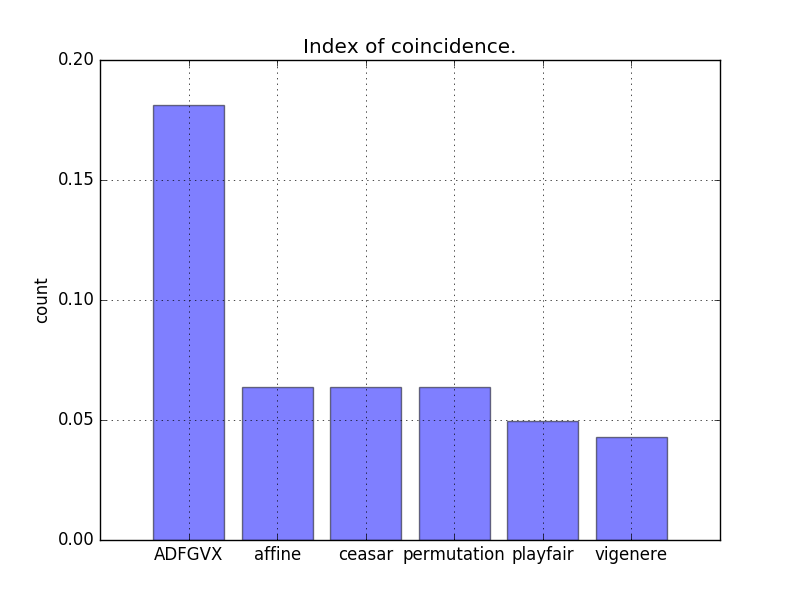
\includegraphics[height=2.5in]{img/iocs.png}
    \end{subfigure}
    \caption{Average index of coincidence.}
    \label{fig:ioc}
\end{figure}

The IC of an English plaintext is approximately $0.065$. The Affine, Caesar and Permutation ciphers are examples of single letter substitution ciphers, where the mapping that determines the encryption of letters is bijective (one-to-one). It is therefore no surprise that the IC of their ciphertexts is the same as the IC of the English plaintexts.

\section{Exploratory data analysis} \label{explore}
%\textcolor{red}{TODO: Do a clustering study. Show scatterplots, bargraphs. Consider ploting variable corelations. https://www.mathworks.com/help/econ/corrplot.html}\\
%\\
One common step before moving on to actual training of the model, is to draw some rough graphs representing the data that will be used for training. This is to see how features interact with each other and to get an idea of how the data clusters.\\
\\
Here I present just one graph to show that the chosen features separate the data in a clear way. I use a subsample of $10\%$ of the data. The features were scaled zero mean and unit variance, and then multidimensional scaling was used to shrink down the data to two dimensions.

\begin{figure}[H]
    \centering
    \begin{subfigure}[h]{0.5\textwidth}
        \centering
        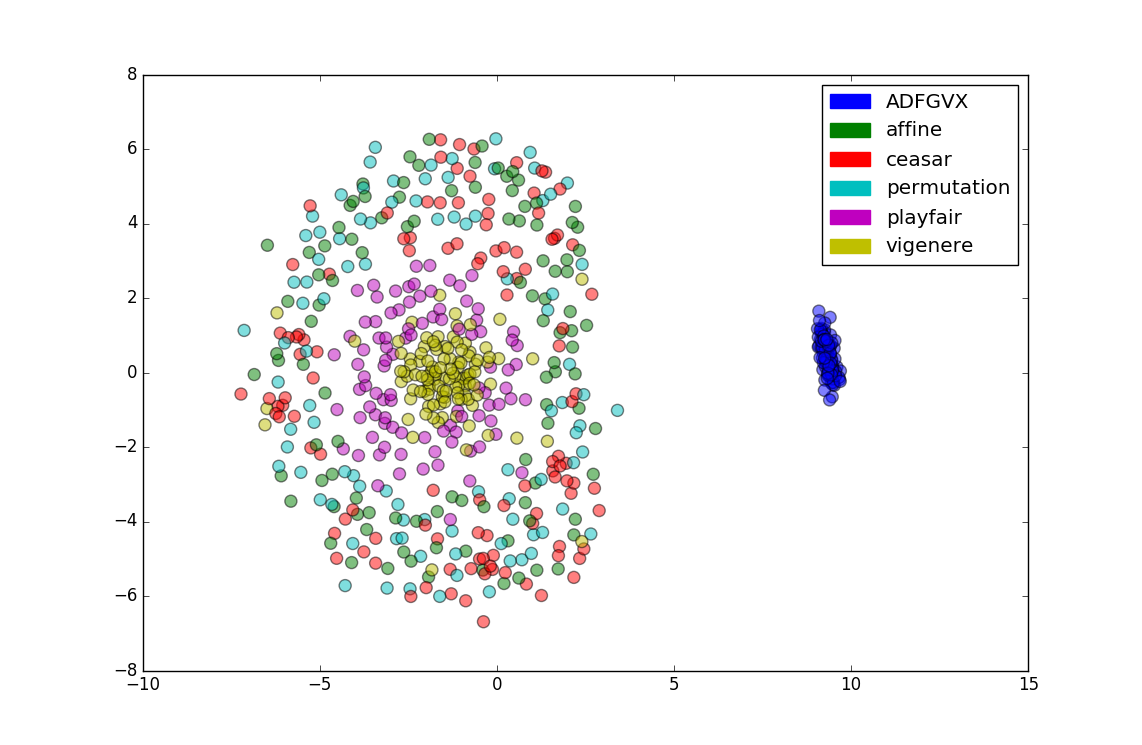
\includegraphics[height=2.5in]{img/mds_features.png}
    \end{subfigure}
    \caption{MDS(multidimensional scaling) used on a subsample of the data.}
    \label{fig:mds}
\end{figure}

In figure \ref{fig:mds} we can see how the ADFGVX cipher is clearly separated from the others. The Vigenere and the Playfair appearing in the inner circles are also separable from the other ciphers, while the Affine, the Caesar and the Permutation ciphers all lay mixed together in the outer most circle. This is an encouraging sight. It tells us that the classifier should produce good results.

\section{Random forest classifier} \label{model}
Random forest is an ensemble method. It works by building multiple simple decision trees on different subsamples of the data and than combining the results to produce a stronger model. It can be used for classification or regression. We will not go into detail about the workings of the decision tree and random forest techniques, since this is a broad topic and it is not the main focus of this report. We advise the reader to learn more in \cite{breiman2001random}. For now it suffices to say that this is a robust machine learning technique that works well on different domains in data science. The main parameter of the random forest is the number of decision trees built. It generally holds that more is better and we usually build as much trees as our computing capabilities allow us, however the accuracy of the model is expected to stop improving substantially at some point.

\begin{figure}[H]
    \centering
    \begin{subfigure}[h]{0.5\textwidth}
        \centering
        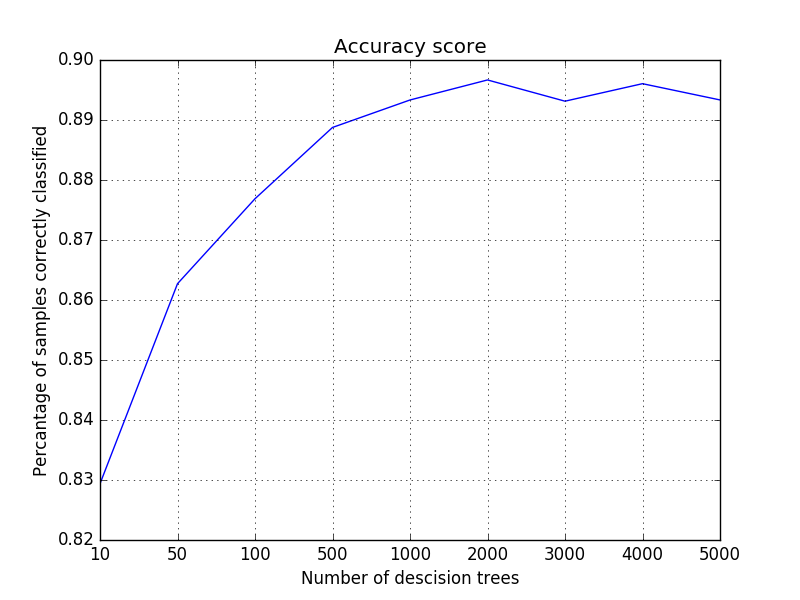
\includegraphics[height=2.5in]{img/accuracy_rf.png}
    \end{subfigure}
    \caption{Determining the optimal number of decision trees in the random forest.}
    \label{fig:acc_rf}
\end{figure}

On graph \ref{fig:acc_rf} we can see how the accuracy score of the random forest changes as we increase the number of decision trees in the forest. We can see that the accuracy of the model does not change significantly for more that $2000$ decision trees. The score was calculated on the training set using a $5$-fold cross validation. 

\section{Results} \label{results}
Training a random forest on the train set of the data, building $2000$ decision trees, I obtained an average accuracy of around $92\%$ on the test set.

\begin{table}[H]
  \begin{center}
    \begin{tabular}{ c | c c c c }
          & \multicolumn{4}{c}{} \\
          & precision     & recall     & f1-score    & support \\
      \hline
      ADFGVX		&1.00	&1.00	&1.00	&195 \\
      Affine		&0.73	&0.77	&0.75	&182 \\
      Caesar      	&0.91	&0.99	&0.95	&212 \\
      Permutation   &0.83	&0.75	&0.79	&210 \\
      Playfair      &1.00	&1.00	&1.00	&208 \\
      Vigenere      &1.00   &0.95	&0.98	&193 \\
      \hline
      avg/total		&0.91	&0.91	&0.91	&1200 \\
    \end{tabular}
  \end{center}
  \caption{Classification report showing the main classification metrics.}
  \label{tab:rf_score}
\end{table}

Table \ref{tab:rf_score} shows some of the more common classification metrics for one specific run on the random forest classifier. Precision tells us the fraction of samples classified as some class that actually belong to this class, while recall or sensitivity tells us the fraction of samples from some class that were classified to be in this class. Example: All of the samples predicted to be Vigenere, were in fact Vigenere so the precision for the Vigenere class is $1.00$, however $9$ of the Vigenere samples were predicted to be Caesar so the recall is only $0.95$. The $f1$-score is the harmonic mean of precision and recall, calculated with the formula 
$$F_{1} = 2 \frac{\rm{precision} \cdot \rm{recall}}{\rm{precision} + \rm{recall}}$$ and support simply tells us how many samples of the class were in the test set. Table \ref{tab:conf_matrix} shows the confusion matrix of the classification.

\begin{table}[H]
  \begin{center}
    \begin{tabular}{| c | c | c | c | c | c | c |}
      \hline
      				&ADFGVX &Affine &Caesar &Permutation &Playfair &Vigenere\\
      \hline
      ADFGVX		&195	&0		&0	    &0			 &0		   &0\\
      \hline
      Affine		&0		&141	&11	    &30 		 &0 	   &0\\
      \hline
      Caesar      	&0		&1		&210	&1	 		 &0 	   &0\\
      \hline
      Permutation   &0		&44		&0		&166 		 &0		   &0\\
      \hline
      Playfair      &0		&0		&0		&0	 		 &208 	   &0\\
      \hline
      Vigenere      &0	    &0		&9		&0	 		 &0 	   &184\\
      \hline
    \end{tabular}
  \end{center}
  \caption{Confusion matrix of the classification.}
  \label{tab:conf_matrix}
\end{table}

We can see that the samples of ADFGVX and Playfair ciphers were all correctly classified and only $9$ out of the $196$ samples of the Vigenere cipher were classified as a Caesar cipher. The classifier however had some problems with the classification of the Affine, Caesar and Permutation ciphers. Out of $182$ samples of the Affine cipher in the test set, $11$ were classified as Caesar and $30$ as Permutation. Out of $212$ samples of the Caesar cipher, $1$ sample was classified as Affine and $1$ as Permutation. Lastly out of $210$ samples of the Permutation cipher, $44$ were classified as Affine.

\section{Framework and Conclusions} \label{frame_conclusion}
For this project I used the Python programming language. I used Pycipher library \cite{pycipher} to encrypt the plaintexts and Scikit-Learn library \cite{scikit-learn} to sample the data, train/tune the model and interpret the results. For the generation of graphs I used the Matplotlib library \cite{Hunter:2007}. For the description of the ciphers I relied on lecture notes from the subject Cryptography and Computer Security taught by prof. Jurišič at the Faculty of Informatics, practical cryptography website \cite{practicalCrypto} and Stinson's book \cite{stinson2005cryptography}.\\
\\
The classification results are encouraging. Using a limited number of fairly simple features we are able to build a model that exhibits an average classification score higher that $90\%$ and it is able to distinguish even between ciphers that use similar encryption rules. To go further and attempt classification of modern ciphers like DES and AES one has to approach the problem with a bit more care. The patterns there are not so clearly visible and by using simple features like the distribution of letters we are not able to distinguish between modern ciphers. Instead more advanced techniques like the ones used in \cite{sivagurunathan2010classification} and \cite{decipher} should be employed.

\bibliographystyle{plain}
\bibliography{sample}

\end{document} 
